% Slide 5, idea 2. Plan B lists 16 changes, 3 fit the time, the people and the budget, and the
% AI picks the free swap. The program before and after, on a 5 pm to 6 pm axis, with the
% projector expected at 5.25. Drawn at final size, 18.4 x 9.6 cm. Facts from dev01.json,
% campus_showcase.evaluator.json and the storyboard ("ranks first of 3 feasible, 13 rejected").
\documentclass[border=1pt]{standalone}
% Shared style of every Plan B figure (the deck, the poster and the documentation).
% Type is near-black and grey on white. UMB blue is the brand and the system. One warm accent
% marks tension only (the incoming message, the clock). Green marks only an accepted receipt or
% a met run. Square corners, thin rules, no shadows, no gradients.
\usepackage[T1]{fontenc}
\usepackage[scaled]{helvet}
\renewcommand{\familydefault}{\sfdefault}
\usepackage{tikz}
\usepackage{pgfplots}
\pgfplotsset{compat=1.18}
\usepackage{fontawesome5}
\hyphenpenalty=10000
\exhyphenpenalty=10000
\usetikzlibrary{arrows.meta,positioning,calc,fit,backgrounds}

% Colours
\definecolor{primary}{HTML}{08457E}   % UMB blue: the system, Plan B's own policy
\definecolor{primarysoft}{HTML}{E7EEF5}
\definecolor{accent}{HTML}{FF791F}    % tension only: the message, the gap, the one missed run
\definecolor{accentsoft}{HTML}{FFEBDC}
\definecolor{umbblue}{HTML}{005A8B}   % UMB blue: the three idea marks and structure
\definecolor{navy}{HTML}{132245}      % title bands, the receipt, the dark close
\definecolor{ground}{HTML}{EEF2F6}    % the light blue-grey ground behind white cards
\definecolor{ok}{HTML}{2E7D32}        % an accepted receipt, a met run
\definecolor{oksoft}{HTML}{E5F1E6}
\definecolor{ink}{HTML}{1F1F1F}
\definecolor{muted}{HTML}{6B6B6B}
\definecolor{quiet}{HTML}{9A9A9A}     % other policies, context
\definecolor{rulegrey}{HTML}{C4C4C4}
\definecolor{gridgrey}{HTML}{E4E4E4}
\definecolor{faint}{HTML}{F4F4F4}

\tikzset{
  >={Stealth[length=2.4mm,width=1.8mm]},
  every picture/.style={line cap=butt, line join=miter},
  % text styles
  hd/.style={font=\bfseries, text=ink, align=left},
  sub/.style={text=muted, align=left},
  % shapes: square or 1 pt corners, thin rules
  card/.style={draw=rulegrey, line width=0.5pt, fill=white, rounded corners=1pt, inner sep=5pt, align=left, text=ink},
  sys/.style={draw=primary, line width=0.8pt, fill=white, rounded corners=1pt, inner sep=5pt, align=center, text=ink},
  sysfill/.style={draw=primary, line width=0.8pt, fill=primary, rounded corners=1pt, inner sep=5pt, align=center, text=white},
  warm/.style={draw=accent, line width=0.8pt, fill=accentsoft, rounded corners=1pt, inner sep=5pt, align=left, text=ink},
  receipt/.style={draw=ok, line width=0.8pt, fill=oksoft, rounded corners=1pt, inner sep=5pt, align=left, text=ink},
  planned/.style={draw=muted, line width=0.6pt, dash pattern=on 3pt off 2pt, fill=white, rounded corners=1pt, inner sep=5pt, align=left, text=muted},
  % connectors
  link/.style={->, draw=muted, line width=0.6pt},
  syslink/.style={->, draw=primary, line width=0.9pt},
  oklink/.style={->, draw=ok, line width=0.9pt},
  warmlink/.style={->, draw=accent, line width=0.9pt},
  nextlink/.style={->, draw=muted, line width=0.6pt, dash pattern=on 3pt off 2pt},
}

% Charts: a real axis, few light gridlines, no frame on the top and right.
\pgfplotsset{
  planb/.style={
    axis line style={draw=muted, line width=0.5pt},
    tick style={draw=muted, line width=0.5pt},
    major tick length=3pt,
    tick label style={text=ink, /pgf/number format/assume math mode=true},
    label style={text=ink},
    title style={font=\bfseries, text=ink},
    grid style={draw=gridgrey, line width=0.4pt},
    every axis plot/.append style={line width=0.6pt},
    legend style={draw=none, fill=none, text=ink},
    legend cell align=left,
  },
}

% The three idea marks, the same in the deck, the poster and the report.
% 1 Check the fact (a magnifier), 2 Pick only what fits (a funnel that keeps what fits),
% 3 Leave a receipt (a receipt slip). Always in UMB blue unless the panel is navy.
\providecommand{\markcheck}{\faSearch}
\providecommand{\markfits}{\faFilter}
\providecommand{\markreceipt}{\faReceipt}
% The three points of "Why Plan B": safer shows the three marks together, more flexible a laptop,
% more personal a set of sliders.
\providecommand{\marksafer}{\faSearch\,\faFilter\,\faReceipt}
\providecommand{\markflexible}{\faLaptop}
\providecommand{\markpersonal}{\faSlidersH}

\begin{document}
\fontsize{12}{14}\selectfont
\begin{tikzpicture}[x=1cm, y=1cm, line join=round]
  \def\W{18.33}\def\H{9.53}
  \useasboundingbox (0,0) rectangle (\W,\H);
  % ------------------------------------------------------------ the 16 changes
  \def\ts{1.52}\def\tg{0.22}
  \node[text=ink, font=\fontsize{22}{26}\selectfont\bfseries] at (3.37,8.95) {16 changes, 3 fit};
  \foreach \r in {0,...,3}{\foreach \c in {0,...,3}{
    \pgfmathsetmacro{\x}{\c*(\ts+\tg)}
    \pgfmathsetmacro{\y}{8.05-\r*(\ts+\tg)}
    \fill[gridgrey, rounded corners=4pt] (\x,\y) rectangle (\x+\ts,\y-\ts);
  }}
  \foreach \r/\c in {0/1, 1/3, 3/0}{
    \pgfmathsetmacro{\x}{\c*(\ts+\tg)}
    \pgfmathsetmacro{\y}{8.05-\r*(\ts+\tg)}
    \fill[umbblue, rounded corners=4pt] (\x,\y) rectangle (\x+\ts,\y-\ts);
  }
  % the AI's pick, ringed
  \pgfmathsetmacro{\px}{3*(\ts+\tg)}
  \pgfmathsetmacro{\py}{8.05-1*(\ts+\tg)}
  \draw[navy, line width=2.4pt, rounded corners=6pt] (\px-0.13,\py+0.13) rectangle (\px+\ts+0.13,\py-\ts-0.13);
  \pgfmathsetmacro{\pyc}{\py-\ts/2}
  \draw[navy, line width=2.2pt, -{Stealth[length=4.5mm,width=4mm]}] (\px+\ts+0.25,\pyc) -- (9.45,\pyc);
  \node[anchor=south, text=navy, font=\fontsize{16}{19}\selectfont\bfseries] at ({(\px+\ts+9.45)/2+0.25},\pyc+0.15) {AI's pick};

  % ------------------------------------------------------------ the program, before and after
  \def\xa{9.95}\def\xb{18.25}
  \pgfmathsetmacro{\s}{(\xb-\xa)/60}
  \newcommand{\tx}[1]{\xa+#1*\s}
  % axis
  \draw[muted, line width=0.8pt] (\xa,1.15) -- (\xb,1.15);
  \foreach \t in {0,60}{\draw[muted, line width=0.8pt] ({\xa+\t*\s},1.15) -- ({\xa+\t*\s},0.95);}
  \node[anchor=north west, inner sep=0pt, text=ink, font=\fontsize{16}{19}\selectfont] at (\xa-0.05,0.85) {5 pm};
  \node[anchor=north east, inner sep=0pt, text=ink, font=\fontsize{16}{19}\selectfont] at (\xb+0.04,0.85) {6 pm};
  % rows
  \def\bh{2.4}
  \def\yB{5.05}\def\yA{1.6}
  \node[anchor=south west, text=ink, font=\fontsize{18}{21}\selectfont\bfseries, inner sep=0pt] at (\xa,\yB+\bh+0.22) {Before};
  \node[anchor=south west, text=ink, font=\fontsize{18}{21}\selectfont\bfseries, inner sep=0pt] at (\xa,\yA+\bh+0.22) {After};
  \def\g{0.04}
  % the projector, expected at 5.25, drawn behind the bars
  \draw[accent, line width=1.6pt] ({\xa+25*\s},1.15) -- ({\xa+25*\s},8.55);
  % before
  \fill[rulegrey] ({\xa+0*\s+\g},\yB) rectangle ({\xa+10*\s-\g},\yB+\bh);
  \filldraw[fill=accentsoft, draw=accent, line width=1.2pt] ({\xa+10*\s+\g+0.03},\yB+0.02) rectangle ({\xa+30*\s-\g-0.03},\yB+\bh-0.02);
  \node[text=ink, font=\fontsize{16}{19}\selectfont\bfseries] at ({\xa+17.5*\s},\yB+\bh/2) {Demos};
  \fill[primarysoft] ({\xa+30*\s+\g},\yB) rectangle ({\xa+50*\s-\g},\yB+\bh);
  \node[text=umbblue, align=center, font=\fontsize{16}{19}\selectfont\bfseries] at ({\xa+40*\s},\yB+\bh/2) {Skills\\exchange};
  \fill[rulegrey] ({\xa+50*\s+\g},\yB) rectangle ({\xa+60*\s},\yB+\bh);
  % after
  \fill[rulegrey] ({\xa+50*\s+\g},\yA) rectangle ({\xa+60*\s},\yA+\bh);
  \fill[rulegrey] ({\xa+0*\s+\g},\yA) rectangle ({\xa+10*\s-\g},\yA+\bh);
  \fill[primarysoft] ({\xa+10*\s+\g},\yA) rectangle ({\xa+30*\s-\g},\yA+\bh);
  \node[text=umbblue, align=center, font=\fontsize{16}{19}\selectfont\bfseries] at ({\xa+20*\s},\yA+\bh/2) {Skills\\exchange};
  \fill[umbblue] ({\xa+30*\s+\g},\yA) rectangle ({\xa+50*\s-\g},\yA+\bh);
  \node[text=white, font=\fontsize{18}{21}\selectfont\bfseries] at ({\xa+40*\s},\yA+\bh/2) {Demos};
  % the projector mark
  \node[anchor=south east, text=accent, font=\fontsize{22}{22}\selectfont, inner sep=0pt] at ({\xa+25*\s-0.1},8.68) {\faVideo};
  \node[anchor=south west, text=accent, font=\fontsize{18}{21}\selectfont\bfseries, inner sep=0pt] at ({\xa+25*\s+0.14},8.68) {5.25 pm};
\end{tikzpicture}
\end{document}
